\documentclass[conference]{IEEEtran}
\IEEEoverridecommandlockouts
% The preceding line is only needed to identify funding in the first footnote. If that is unneeded, please comment it out.
\usepackage[utf8]{inputenc}
\usepackage[spanish]{babel}
\usepackage{cite}
\usepackage{amsmath,amssymb,amsfonts}
\usepackage{algorithmic}
\usepackage{hyperref}
\usepackage{graphicx}
\usepackage{textcomp}
\usepackage{xcolor}
\def\BibTeX{{\rm B\kern-.05em{\sc i\kern-.025em b}\kern-.08em
    T\kern-.1667em\lower.7ex\hbox{E}\kern-.125emX}}
\begin{document}

\title{Sistema Inteligente de Monitoreo y Gestión del Consumo de Agua en Tiempo Real}

\author{\IEEEauthorblockN{Santiago Llerena Lanchero}
    \IEEEauthorblockA{\textit{Dpto. de Ingeniería de Sistemas} \\
        \textit{Universidad del Norte}\\
        Barranquilla, Colombia \\
        \href{slanchero@uninorte.edu.co}{\texttt{slanchero@uninorte.edu.co}}}
    \and
    \IEEEauthorblockN{Cristian Cubillos Torres}
    \IEEEauthorblockA{\textit{Dpto. de Ingeniería de Sistemas} \\
        \textit{Universidad del Norte}\\
        Barranquilla, Colombia \\
        \href{cccubillos@uninorte.edu.co}{\texttt{cccubillos@uninorte.edu.co}}}
    \and
    \IEEEauthorblockN{Santiago Cardona Julio}
    \IEEEauthorblockA{\textit{Dpto. de Ingeniería de Sistemas} \\
        \textit{Universidad del Norte}\\
        Barranquilla, Colombia \\
        \href{sacardona@uninorte.edu.co}{\texttt{sacardona@uninorte.edu.co}}}
}

\maketitle

\begin{abstract}
    This document is a model and instructions for \LaTeX.
    This and the IEEEtran.cls file define the components of your paper [title, text, heads, etc.]. *CRITICAL: Do Not Use Symbols, Special Characters, Footnotes,
    or Math in Paper Title or Abstract.
\end{abstract}

\begin{IEEEkeywords}
    component, formatting, style, styling, insert
\end{IEEEkeywords}

\section{Introducción}
El agua es un recurso vital para la vida humana y su gestión eficiente se ha
convertido en un tema crítico en el contexto actual de cambio climático y
crecimiento poblacional. Según la Organización de las Naciones Unidas (ONU),
más del 40\% de la población mundial vive en regiones con estrés hídrico, y se
estima que para 2050 esta cifra aumentará significativamente si no se toman
medidas adecuadas (ONU, 2021). En este sentido, el monitoreo y control del
consumo de agua en los hogares se presenta como una estrategia clave para
promover el uso responsable de este recurso.

El Internet de las Cosas (IoT, por sus siglas en inglés) ha emergido como una
tecnología transformadora en la gestión de recursos, permitiendo la
interconexión de dispositivos y la recopilación de datos en tiempo real. A
través de sensores, microcontroladores y plataformas en la nube, es posible
crear sistemas inteligentes que no solo monitorean el consumo de agua, sino que
también alertan a los usuarios sobre patrones de uso ineficientes o posibles
fugas. Según Gartner (2020), el número de dispositivos IoT conectados a nivel
mundial superará los 25 mil millones para 2025, lo que refleja el potencial de
esta tecnología para optimizar procesos y mejorar la calidad de vida.

Este proyecto tiene como objetivo desarrollar un sistema de monitoreo y alerta
del consumo de agua en una vivienda, utilizando tecnologías IoT. El sistema
integrará un sensor de flujo de agua, un microcontrolador y una aplicación
móvil para visualizar los datos en tiempo real y enviar notificaciones en caso
de detectar anomalías, como fugas o consumos excesivos. Además, se implementará
un mecanismo de control automático que permita cerrar el flujo de agua en
situaciones de emergencia. Este enfoque no solo contribuye a la conservación
del agua, sino que también ofrece a los usuarios una herramienta práctica y
accesible para gestionar su consumo de manera más eficiente directamente desde
sus dispositivos móviles.

\section{Problema}

\begin{figure*}[ht]
    \centering
    \includegraphics[width=\textwidth]{Arbol del problema.png}
    \caption{Árbol del Problema}
    \label{fig: Arbol del problema}
\end{figure*}

El agua es un recurso esencial para la vida y el desarrollo de las sociedades;
sin embargo, su disponibilidad se ve cada vez más comprometida debido al
crecimiento poblacional, la urbanización acelerada y los efectos del cambio
climático. Según la Organización de las Naciones Unidas para la Educación, la
Ciencia y la Cultura (UNESCO, 2023), aproximadamente el 25\% de la población
mundial vive en países que enfrentan estrés hídrico severo, y se prevé que esta
cifra aumente en las próximas décadas. En este contexto, la gestión eficiente
del agua en los hogares se ha convertido en un desafío crítico, ya que el
consumo doméstico representa una parte significativa del uso total de este
recurso.

En muchas viviendas, el consumo de agua no se monitorea de manera sistemática,
lo que dificulta la identificación de patrones de uso ineficientes o la
detección temprana de fugas. Según un estudio realizado por la Environmental
Protection Agency (EPA, 2022), una fuga promedio en un hogar puede desperdiciar
hasta 10,000 galones de agua al año, lo que no solo impacta negativamente en el
medio ambiente, sino que también genera costos económicos significativos para
las familias. Además, la falta de conciencia sobre el consumo real de agua
limita la capacidad de los usuarios para adoptar medidas que promuevan un uso
más sostenible.

Aunque existen tecnologías que permiten medir el consumo de agua, muchas de
estas soluciones son costosas, complejas de implementar o no están integradas
con sistemas de alerta y control en tiempo real. Esto limita su accesibilidad y
efectividad, especialmente en regiones con recursos económicos limitados. Por
otro lado, el Internet de las Cosas (IoT) ha demostrado ser una herramienta
poderosa para la gestión de recursos, pero su aplicación en el monitoreo
doméstico del agua aún no ha sido ampliamente adoptada, a pesar de su potencial
para transformar la manera en que interactuamos con este recurso.

En este escenario, surge la necesidad de desarrollar un sistema accesible y
eficiente que permita monitorear el consumo de agua en tiempo real, detectar
anomalías como fugas o consumos excesivos, y notificar a los usuarios para que
tomen acciones correctivas. Este sistema no solo contribuiría a la conservación
del agua, sino que también empoderaría a los hogares para gestionar su consumo
de manera más consciente y responsable.

\section{Justificación}

El desarrollo de un sistema de monitoreo y alerta del consumo de agua en
viviendas, basado en el Internet de las Cosas (IoT), se justifica por su
relevancia en tres aspectos fundamentales: ambiental, económico y social. En un
mundo donde la escasez de agua se ha convertido en un problema global, es
imperativo implementar soluciones tecnológicas que promuevan un uso más
eficiente y sostenible de este recurso.

\subsection{Justificación Ambiental }

El agua es un recurso finito y esencial para la vida, pero su disponibilidad
está disminuyendo debido al cambio climático, la contaminación y la
sobreexplotación. Según el World Resources Institute (WRI, 2023), más de 2 mil
millones de personas viven en países con alto estrés hídrico, y se estima que
para 2040, una cuarta parte de la población mundial enfrentará escasez severa
de agua. En este contexto, la implementación de sistemas que permitan
monitorear y controlar el consumo de agua en los hogares contribuye
directamente a la conservación de este recurso, reduciendo el desperdicio y
promoviendo prácticas más sostenibles.

\subsection{Justificación Económica }

El desperdicio de agua no solo tiene un impacto ambiental, sino también
económico. De acuerdo con la Environmental Protection Agency (EPA, 2022), una
fuga doméstica promedio puede desperdiciar hasta 10,000 galones de agua al año,
lo que se traduce en un aumento significativo en las facturas de agua para las
familias. Un sistema de monitoreo y alerta permite detectar fugas y consumos
excesivos en tiempo real, lo que ayuda a los usuarios a tomar medidas
inmediatas y evitar gastos innecesarios. Además, la adopción de tecnologías IoT
en el hogar puede incrementar el valor de la propiedad y reducir costos a largo
plazo.

\subsection{Justificación Social }

La falta de conciencia sobre el consumo de agua es un problema común en muchas
comunidades. Un sistema que proporcione datos en tiempo real y notificaciones
sobre el uso del agua empodera a los usuarios para tomar decisiones informadas
y adoptar hábitos más responsables. Además, este tipo de tecnología puede ser
especialmente útil en regiones con acceso limitado a servicios de agua potable,
donde la gestión eficiente del recurso es crucial para garantizar su
disponibilidad. Según la UNESCO (2023), la educación y la tecnología son
herramientas clave para fomentar una cultura de sostenibilidad y
responsabilidad en el uso del agua.

\subsection{Innovación Tecnológica}

El uso del Internet de las Cosas (IoT) en este proyecto representa una
innovación significativa, ya que integra sensores, microcontroladores y
plataformas en la nube para ofrecer una solución accesible y escalable. A
diferencia de los sistemas tradicionales de medición de agua, este enfoque
permite la visualización remota de datos, la generación de alertas y el control
automático del flujo de agua, lo que lo convierte en una herramienta versátil y
eficiente para la gestión doméstica del agua.

En conclusión, este proyecto no solo aborda un problema crítico como es la
gestión del agua, sino que también aprovecha las ventajas de la tecnología IoT
para ofrecer una solución innovadora, accesible y de alto impacto. Su
implementación contribuirá a la conservación del agua, al ahorro económico y a
la promoción de una cultura de sostenibilidad en los hogares.

\section{Objetivos}
\subsection{Objetivo General}
Desarrollar un sistema inteligente de monitoreo y gestión del consumo de agua
basado en tecnologías IoT, sensores de flujo y almacenamiento en la nube, que
permita visualizar el consumo en tiempo real, detectar anomalías y promover el
ahorro del recurso hídrico mediante alertas y control automático.
\subsection{Objetivos específicos}
\begin{enumerate}
    \item Realizar una revisión de literatura sobre el uso de IoT, sensores de flujo de
          agua, análisis de datos y plataformas en la nube aplicadas a la gestión del
          recurso hídrico.

    \item Diseñar la arquitectura del sistema inteligente, definiendo los componentes
          tecnológicos, la infraestructura de comunicación, el procesamiento de datos y
          el almacenamiento en la nube.

    \item Desarrollar un prototipo funcional que integre sensores de flujo de agua, una
          plataforma de procesamiento de datos y una interfaz de visualización en tiempo
          real.

    \item Validar el prototipo mediante pruebas experimentales con usuarios, evaluando su
          precisión en la detección de anomalías, eficiencia en la transmisión de datos y
          facilidad de uso.

    \item Optimizar el sistema con base en los resultados obtenidos en la validación,
          ajustando su desempeño en términos de detección de fugas, consumo energético y
          experiencia de usuario.

\end{enumerate}

\section{Metodología}
El desarrollo de este proyecto se llevará a cabo bajo la metodología ágil
Scrum, un marco de trabajo ágil que permite desarrollar soluciones complejas
mediante iteraciones cortas y entregas incrementales de valor. El proceso de
desarrollo se organiza en cinco sprints, cada uno con objetivos específicos que
contribuyen a la construcción progresiva del prototipo funcional.\\
\begin{figure}[htbp]
    \centerline{\includegraphics[width=\linewidth]{referencia de metodologia.png}}
    \caption{Marco de trabajo \textit{Scrum} aplicado al desarrollo del sistema.}
    \label{fig}
\end{figure}
\begin{itemize}
    \item \textbf{Sprint 1: Levantamiento de requerimientos y diseño conceptual:} \\
          En esta primera etapa se analiza el contexto del problema, se establecen los requisitos del sistema y se define su alcance. Ademas se realiza un primer diseño de la arquitectura general del sistema, incluyendo esquemas de componentes, flujo de datos y mockup de la aplicacion movil.
          \begin{itemize}
              \item Duración estimada: 2 semanas.
              \item Resultados esperados:
                    \begin{itemize}
                        \item Diseño preliminar de la arquitectura.
                        \item Prototipos básicos de interfaz.
                        \item Backlog inicial del producto.
                    \end{itemize}
          \end{itemize}
    \item \textbf{Sprint 2: Desarrollo del sistema de adquisición y transmisión de datos}\\
          Se implementa la conexión entre los sensores de flujo de agua y el microcontrolador. Se programa el módulo encargado de la medición y se establece la comunicación con el entorno backend o plataforma de recepción de datos.
          \begin{itemize}
              \item Duración estimada: 3 semanas.
              \item Resultados esperados:
                    \begin{itemize}
                        \item Sensor de flujo funcionando e integrado con el microcontrolador.
                        \item Envío estable de datos en tiempo real.
                        \item Pruebas iniciales de transmisión y captura de datos.
                    \end{itemize}
          \end{itemize}
    \item \textbf{Sprint 3: Almacenamiento y visualización}\\
          En este sprint se construye la base de datos para almacenar los registros de consumo. También se desarrollan las interfaces de visualización, orientadas al usuario final, donde se presenten métricas de consumo en tiempo real e históricos.
          \begin{itemize}
              \item Duración estimada: 3 semanas.
              \item Resultados esperados:
                    \begin{itemize}
                        \item Base de datos funcional y conectada al sistema.
                        \item Interfaz gráfica para la consulta del consumo.
                        \item Visualización de datos históricos y actuales.
                    \end{itemize}
          \end{itemize}
    \item \textbf{Sprint 4: Implementación del sistema de alertas y control}\\
          Se incorpora el módulo que detecta patrones de consumo anómalos y genera alertas automáticas. También se trabaja en la lógica de cierre automático del flujo en caso de fugas o uso excesivo, conectando el sistema con un actuador físico.
          \begin{itemize}
              \item Duración estimada: 2 semanas.
              \item Resultados esperados:
                    \begin{itemize}
                        \item Sistema de detección de alertas funcional.
                        \item Mecanismo de cierre automático probado.
                        \item Integración entre módulo de control y monitoreo.
                    \end{itemize}
          \end{itemize}
    \item \textbf{Sprint 5: Pruebas finales, validación y mejoras}\\
          Durante el sprint final, se validan todos los módulos implementados en conjunto. Se realizan pruebas de integración y se ajustan detalles de rendimiento.
          \begin{itemize}
              \item Duración estimada: 1 semana.
              \item Resultados esperados: Sistema integrado y operativo.
          \end{itemize}

\end{itemize}

\section{MARCO TEORICO}
La creciente presión sobre los recursos hídricos a nivel global ha impulsado la necesidad de desarrollar sistemas más eficientes para su gestión. Según el World Resources Institute (2023), más de 50 países enfrentarán estrés hídrico extremo para 2040, situación que se agrava por las pérdidas en las redes de distribución que en algunos casos superan el 40\% del agua tratada \cite{c21}. En este contexto, la implementación de sistemas inteligentes de monitoreo se presenta como una solución fundamental para abordar estos desafíos. \\

La Organización de las Naciones Unidas (2021) ha destacado que las tecnologías digitales aplicadas a la gestión del agua pueden contribuir significativamente al cumplimiento del Objetivo de Desarrollo Sostenible 6 (Agua limpia y saneamiento) \cite{c17}. Particularmente, los sistemas en tiempo real permiten una respuesta inmediata ante irregularidades en el consumo, fugas o contaminación del recurso hídrico. \\

Los primeros sistemas de medición de consumo de agua se limitaban a medidores mecánicos que requerían lectura manual periódica. Saseendran y Nithya (2016) documentan cómo esta aproximación presentaba importantes limitaciones en términos de frecuencia de medición y detección de anomalías \cite{c6}. La transición hacia sistemas automatizados comenzó con la incorporación de tecnologías de telemetría básica, que si bien permitían lecturas remotas, carecían de capacidades analíticas avanzadas. \\

El desarrollo del Internet de las Cosas marcó un punto de inflexión en esta evolución. Como señalan Di Mauro et al. (2019), la integración de sensores inteligentes con capacidades de conectividad ha permitido pasar de simples sistemas de medición a plataformas integrales de gestión \cite{c8}. Estos avances han sido particularmente relevantes en el ámbito urbano, donde la complejidad de las redes de distribución requiere soluciones más sofisticadas.\\

Khan et al. (2020) proponen un diseño basado en IoT que utiliza sensores de
flujo para medir el consumo de agua y transmitir los datos a una plataforma
centralizada, facilitando la toma de decisiones \cite{c2}. Por su parte,
Gaikwad et al. (2020) desarrollaron un medidor inteligente que no solo registra
el consumo, sino que también alerta sobre anomalías en el suministro \cite{c3}. \\

\section{MARCO CONCEPTUAL}
\subsection*{\textbf{Internet de las Cosas (IoT)}}
El Internet de las Cosas (IoT) es una tecnología que permite la conexión de dispositivos físicos a través de redes digitales con el fin de capturar, transmitir y procesar datos del entorno en tiempo real. Esta conectividad posibilita el monitoreo y control de variables a distancia, lo cual es fundamental en aplicaciones donde se requiere supervisión continua y respuestas automáticas. En el contexto del recurso hídrico, el IoT se ha consolidado como una herramienta eficaz para gestionar el consumo y la distribución de agua, optimizando su uso mediante sensores, actuadores, microcontroladores y plataformas en la nube (Kumar et al., 2022; Razaque \& Elleithy, 2019).
\subsection*{\textbf{Sensores de Flujo y Monitoreo Hídrico}}
Los sensores de flujo permiten registrar la cantidad de agua que circula a través de una tubería en tiempo real. Estos sensores, cuando son integrados en sistemas inteligentes, permiten identificar patrones de consumo, detectar fugas o uso anómalo, y realizar ajustes automáticos. Su funcionamiento puede basarse en principios mecánicos, ultrasónicos o electromagnéticos. Además, al conectarse con sistemas IoT, los datos pueden ser visualizados remotamente, lo que mejora la capacidad de reacción ante emergencias o comportamientos ineficientes del sistema (Thakur et al., 2023).
\subsection*{\textbf{Calidad del Agua y Monitoreo en Tiempo Real}}
La calidad del agua es un indicador fundamental para la salud pública y la sostenibilidad ambiental. Variables como el pH, la turbidez, la temperatura, el oxígeno disuelto y la presencia de metales pesados pueden ser medidas utilizando sensores especializados conectados a sistemas IoT. El monitoreo continuo de estos parámetros permite detectar de forma temprana eventos de contaminación y tomar medidas correctivas sin demoras. La integración de estos sistemas con redes de comunicación permite que los datos sean procesados y analizados de manera inmediata, lo cual reduce riesgos asociados al consumo de agua no apta (Wu et al., 2023; Sharma et al., 2021).
\subsection*{\textbf{Automatización en la Gestión del Agua}}
La automatización en los sistemas de gestión hídrica implica el uso de tecnologías que permiten operar válvulas, bombas y otros mecanismos de forma autónoma, en función de variables monitoreadas en tiempo real. Esta característica resulta esencial para mejorar la eficiencia en el uso del agua, especialmente en zonas con alta demanda o recursos limitados. La automatización puede ser controlada localmente mediante microcontroladores, o remotamente a través de plataformas IoT, lo que facilita su implementación en entornos rurales o de difícil acceso (Ramesh \& Chinnadurai, 2022).
\subsection*{\textbf{Interfaces de Usuario y Visualización de Datos}}
Un componente fundamental en los sistemas inteligentes de gestión hídrica es la capacidad de presentar la información recolectada de manera clara e intuitiva para el usuario final. Las interfaces gráficas, ya sea en aplicaciones móviles o plataformas web, permiten al usuario tomar conciencia de su consumo, recibir alertas, acceder a reportes históricos, y ajustar su comportamiento. La retroalimentación visual y en tiempo real se ha identificado como un factor clave para fomentar prácticas más sostenibles en el uso del recurso (Chakraborty et al., 2021).
\subsection*{\textbf{Seguridad y Confiabilidad en Sistemas IoT}}
La incorporación de tecnologías IoT también plantea retos relacionados con la seguridad de la información, la integridad de los datos y la confiabilidad del sistema. Los dispositivos conectados están expuestos a riesgos como accesos no autorizados, interrupciones en la comunicación o manipulación de datos. Por ello, es fundamental implementar medidas de seguridad como autenticación robusta, cifrado de datos y protocolos de respaldo. Un sistema de gestión del agua que opere bajo estas condiciones debe garantizar tanto la precisión de los datos como su disponibilidad continua (Zhou et al., 2023).

\section{ARQUITECTURAS}

\subsection*{\textbf{Arquitectura fisica de la solución}}
La arquitectura física del sistema se basa en una integración eficiente entre hardware IoT y una plataforma de backend ligera. El sensor YF-S201 mide el flujo de agua y transmite los datos al microcontrolador ESP32, que se encarga de procesarlos y enviarlos mediante conexión WiFi al backend desarrollado con NestJs, alojado en una instancia de Azure. Esta base de datos ligera actúa como puente entre el hardware y la aplicación móvil, permitiendo almacenar y consultar datos en tiempo real. El dispositivo móvil del usuario se conecta aL backend usando WebSocket y peticiones HTTP para visualizar el consumo de agua, recibir notificaciones y modificar configuraciones, manteniendo así una comunicación bidireccional entre el usuario y el sistema de monitoreo. Esta arquitectura es ideal para proyectos ligeros y escalables que requieren interacción en tiempo real con dispositivos físicos.
\begin{figure}[!htbp]
\centerline{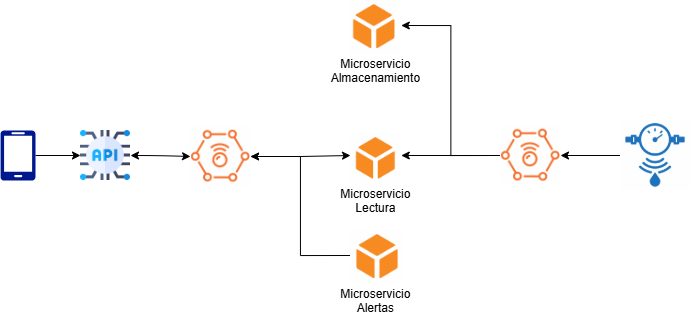
\includegraphics[width=\linewidth,height=210px]{arquitectura_final_ms.png}}
\caption{Arquitectura de flujo del sistema de monitoreo y gestión del consumo de agua.}
    
\end{figure}

La arquitectura física del sistema propuesto está basada en un enfoque orientado a eventos y compuesta por un backend desarrollado con el framework NestJS, estructurado bajo una arquitectura de microservicios desplegados de manera independiente. Esta arquitectura permite escalabilidad, mantenibilidad y procesamiento asíncrono de eventos generados por los sensores de consumo de agua. El sistema está conformado por tres microservicios principales. El primero es el microservicio de almacenamiento de datos, encargado de recibir los datos enviados por los sensores de flujo de agua y persistirlos en la base de datos. Este microservicio está conectado a un event broker que se encarga de recibir los eventos provenientes de los sensores y de notificar a los demás componentes para su correspondiente tratamiento. El segundo componente es el microservicio de lectura, responsable de consultar los datos almacenados, procesarlos (por ejemplo, calcular consumo diario o por hora) y enviarlos a la aplicación móvil para su visualización. Este microservicio también se encuentra conectado al event broker para recibir actualizaciones en tiempo real cuando llegan nuevos datos, lo que permite reflejar los cambios en las gráficas sin necesidad de recarga manual. Finalmente, el microservicio de análisis y notificaciones tiene como función principal analizar los datos históricos o en tiempo real, detectar patrones o eventos relevantes como consumos inusuales, y generar alertas o notificaciones personalizadas para el usuario.

Para garantizar una comunicación eficiente y desacoplada entre componentes, se han implementado dos canales de eventos. El primero es el canal de eventos de sensores, que conecta los microservicios de almacenamiento y lectura con el event broker encargado de manejar los eventos provenientes del dispositivo IoT. Este canal garantiza la llegada y tratamiento de los datos en tiempo real. El segundo canal es el canal de eventos para la aplicación móvil, que conecta los microservicios de lectura y notificaciones con un segundo event broker, el cual establece comunicación con el API Gateway mediante WebSocket. Esta conexión permite enviar actualizaciones instantáneas a la aplicación móvil del usuario, asegurando una experiencia interactiva y sin latencia percibida. Gracias a esta arquitectura orientada a eventos, el sistema puede responder rápidamente ante nuevos datos, escalar horizontalmente según la carga, y garantizar una alta disponibilidad y eficiencia en el procesamiento de información en tiempo real.

\begin{figure}[!htbp]
\centerline{\includegraphics[width=\linewidth,height=1\textheight,keepaspectratio]{Arquitectura_fisica_ff.png}}
\caption{Arquitectura de software del sistema de monitoreo y gestión del consumo de agua.}
\label{fig}
\end{figure}

\newpage

\subsection*{\textbf{Arquitectura logica de la solución}}
Esta arquitectura basada en eventos permite el monitoreo inteligente del consumo de agua mediante sensores IoT que capturan datos como flujo constante de agua. Los eventos generados por estos sensores se envían a través de un bus de eventos utilizando comunicación ligera como MQTT. Una vez recibidos, estos eventos son procesados por componentes que almacenan la información en bases de datos como MondoDB. Un motor de reglas interpreta los datos para activar acciones como notificaciones o alertas, mientras que los datos también se visualizan en dispositivos móviles para brindar al usuario información clara y en tiempo real sobre su consumo de agua.
\begin{figure}[!htbp]
\centerline{\includegraphics[width=\linewidth,height=380px]{arquitectura_logica_final.png}}
\caption{Arquitectura basada en eventos del sistema de monitoreo y gestión del consumo de agua.}
\label{fig}
\end{figure}






\clearpage

\section{PROTOTIPO}
En esta sección se presenta el prototipo funcional de la solución, enfocado en la interfaz de usuario. Se describen las principales vistas del frontend y las funcionalidades disponibles en cada una, mostrando cómo el usuario puede interactuar con el sistema para visualizar y analizar los datos recolectados.

\subsection*{\textbf{Pantalla de bienvenida}}
Al iniciar la aplicación, se muestra una pantalla de bienvenida donde el usuario puede ingresar su nombre y configurar los límites de consumo de agua diarios y mensuales. Esta configuración inicial permite personalizar la experiencia y establecer umbrales para futuras alertas.



\begin{figure}[htbp]
    \centerline{\includegraphics[width=\linewidth, height=450px]{Prototipo1.jpeg}}
    \caption{Pantalla de bienvenida con configuración inicial de límites de consumo.}
    \label{fig}
\end{figure}

\newpage



\subsection*{\textbf{Vinculación del sensor}}
Al acceder por primera vez, el usuario ve una pantalla en blanco indicando que no hay dispositivos vinculados.
Para comenzar el monitoreo, simplemente debe ingresar el número de serie del sensor en el formulario de vinculación.
Una vez validado, el sistema muestra el dispositivo como activo y listo para enviar datos en tiempo real.


\begin{figure}[htbp]
    \centerline{\includegraphics[width=\linewidth, height=450px]{Prototipo2.jpeg}}
    \caption{Vista inicial del sistema sin dispositivos vinculados.}
    \label{fig}
\end{figure}

\newpage

\begin{figure}[htbp]
    \centerline{\includegraphics[width=\linewidth]{Prototipo3.jpg}}
    \caption{Formulario para ingresar el número de serie del sensor y vincularlo al sistema.}
    \label{fig}
\end{figure}

\begin{figure}[htbp]
    \centerline{\includegraphics[width=\linewidth]{Prototipo4.jpg}}
    \caption{Dispositivo vinculado correctamente, listo para transmitir datos.}
    \label{fig}
\end{figure}


\newpage
\subsection*{\textbf{Pagina principal}}
La pantalla principal de la aplicación permite al usuario visualizar el flujo de agua en tiempo real, acompañado de un resumen rápido con valores clave como el flujo actual, máximo, mínimo y promedio. Justo debajo, se presentan gráficas con información del consumo diario, con opción de navegar por vistas semanales y mensuales. Esta sección brinda una visión completa del comportamiento del consumo de agua en el hogar.

\begin{figure}[htbp]
    \centerline{\includegraphics[width=\linewidth, height=450px]{Prototipo5.jpeg}}
    \caption{Visualización del consumo diario de agua y acceso al mapa de calor mensual.}
    \label{fig}
\end{figure}

\begin{figure}[htbp]
    \centerline{\includegraphics[width=\linewidth, height=450px]{Prototipo6.jpeg}}
    \caption{Resumen rápido del flujo de agua en tiempo real, incluyendo valores mínimo, máximo, promedio y actual.}
    \label{fig}
\end{figure}

\newpage

\section{CONCLUSIÓN}

El proyecto abordó la problemática del uso ineficiente del agua en los hogares mediante el desarrollo de un sistema inteligente de monitoreo basado en tecnologías IoT. A partir del análisis del contexto ambiental y social, se propuso una solución viable que permite a los usuarios visualizar su consumo en tiempo real, recibir alertas ante anomalías y tomar decisiones para reducir el desperdicio.

La implementación del prototipo y su arquitectura modular demostraron que es posible integrar sensores, microcontroladores y plataformas en la nube en una herramienta funcional y escalable. Esta solución no solo contribuye a la conservación del recurso hídrico, sino que también promueve una gestión más consciente y sostenible desde el entorno doméstico.

Los objetivos planteados al inicio del proyecto fueron alcanzados satisfactoriamente. Se realizó una revisión teórica del uso de tecnologías IoT en la gestión hídrica, se diseñó e implementó una arquitectura funcional basada en microservicios y eventos, y se desarrolló un prototipo que integra sensores de flujo, almacenamiento en la nube y una interfaz móvil intuitiva. Además, el sistema fue validado mediante pruebas experimentales que permitieron evaluar su precisión, eficiencia y facilidad de uso, lo que facilitó su posterior optimización en aspectos clave como la detección de anomalías y la experiencia del usuario.

El desarrollo del proyecto se estructuró siguiendo la metodología ágil Scrum, lo que permitió avanzar de forma iterativa y ordenada en la construcción del sistema. A lo largo de los sprints, se abordaron tareas clave como el levantamiento de requerimientos, la integración de sensores y el diseño de la interfaz. Paralelamente, se definieron un marco teórico y conceptual que fundamentaron el uso de tecnologías IoT, sensores de flujo y mecanismos de visualización en tiempo real, asegurando la solidez técnica de la solución. Finalmente, se diseñaron arquitecturas lógicas y físicas que integran hardware, microservicios, almacenamiento en la nube y una aplicación móvil, permitiendo una gestión eficiente y escalable del consumo de agua.

El prototipo desarrollado demuestra la viabilidad técnica y funcional del sistema propuesto. A través de la aplicación móvil, los usuarios pueden monitorear su consumo en tiempo real, recibir alertas ante patrones anómalos y tomar decisiones informadas para mejorar su uso del recurso hídrico. La integración efectiva entre hardware, backend y visualización, validada mediante pruebas, evidencia que esta solución puede escalarse y adaptarse a entornos reales. En consecuencia, el proyecto representa una propuesta factible y de alto impacto para su implementación en hogares, promoviendo un consumo de agua más eficiente, consciente y sostenible.


\section{VALIDACIÓN DEL PROTOTIPO}


\begin{figure}[ht]
    \centerline{\includegraphics[width=\linewidth, height = 174.6px]{ValidacionPrototipo.jpg}}
    \caption{Modelo de evaluacióntipo escala de Likert para la validación del prototipo}
    \label{fig}
\end{figure}

\newpage



\begin{thebibliography}{99}

    \bibitem{c1}
    A. A. S. Chowdhury, Y. Arafat and M. S. Alam, ``IoT-GSM Based Controlling and Monitoring System to Prevent Water Wastage, Water Leakage, and Pollution in the Water Supply,'' \textit{2022 International Conference on Innovations in Science, Engineering and Technology (ICISET)}, Chittagong, Bangladesh, 2022, pp. 567–572. \href{https://doi.org/10.1109/ICISET54810.2022.9775876}{doi:10.1109/ICISET54810.2022.9775876}.

    \bibitem{c2}
    Z. U. Khan et al., ``Design of an IoT-based water flow monitoring system,'' in \textit{Proc. 26th Annual Int. Conf. on Mobile Computing and Networking (MobiCom '20)}, Article 91, 2020. \href{https://doi.org/10.1145/3372224.3418170}{doi:10.1145/3372224.3418170}.

    \bibitem{c3}
    V. Gaikwad, Y. Bagul, A. Sarap and S. Swami, ``IOT based Smart Flow Meter for Smart Cities,'' \textit{2020 IEEE Pune Section Int. Conf. (PuneCon)}, Pune, India, 2020, pp. 138–141. \href{https://doi.org/10.1109/PuneCon50868.2020.9362468}{doi:10.1109/PuneCon50868.2020.9362468}.

    \bibitem{c4}
    G. Ndayisenga et al., ``IoT Based Household Water Consumption Management System,'' \textit{2022 IEEE PES/IAS PowerAfrica}, Kigali, Rwanda, 2022, pp. 1–4. \href{https://doi.org/10.1109/PowerAfrica53997.2022.9905316}{doi:10.1109/PowerAfrica53997.2022.9905316}.

    \bibitem{c5}
    P. B. Agarkar et al., ``Efficient Water Resource Management: An IoT-Based Smart Water Level Monitoring and Control System,'' \textit{2023 4th Int. Conf. on Computation, Automation and Knowledge Management (ICCAKM)}, Dubai, UAE, 2023, pp. 1–5. \href{https://doi.org/10.1109/ICCAKM58659.2023.10449619}{doi:10.1109/ICCAKM58659.2023.10449619}.

    \bibitem{c6}
    S. Saseendran and V. Nithya, ``Automated water usage monitoring system,'' \textit{2016 Int. Conf. on Communication and Signal Processing (ICCSP)}, Melmaruvathur, India, 2016, pp. 99–103. \href{https://doi.org/10.1109/ICCSP.2016.7754501}{doi:10.1109/ICCSP.2016.7754501}.

    \bibitem{c7}
    Z. H. Che Soh et al., ``IoT Water Consumption Monitoring \& Alert System,'' \textit{2018 Int. Conf. on Electrical Engineering and Informatics (ICELTICs)}, Banda Aceh, Indonesia, 2018, pp. 168–172. \href{https://doi.org/10.1109/ICELTICS.2018.8548930}{doi:10.1109/ICELTICS.2018.8548930}.

    \bibitem{c8}
    A. Di Mauro et al., ``An IoT System for Monitoring and Data Collection of Residential Water End-Use Consumption,'' \textit{2019 28th Int. Conf. on Computer Communication and Networks (ICCCN)}, Valencia, Spain, 2019, pp. 1–6. \href{https://doi.org/10.1109/ICCCN.2019.8847120}{doi:10.1109/ICCCN.2019.8847120}.

    \bibitem{c9}
    S. S. Siddula, P. Babu and P. C. Jain, ``Water Level Monitoring and Management of Dams using IoT,'' \textit{2018 3rd Int. Conf. on Internet of Things: Smart Innovation and Usages (IoT-SIU)}, Bhimtal, India, 2018, pp. 1–5. \href{https://doi.org/10.1109/IoT-SIU.2018.8519843}{doi:10.1109/IoT-SIU.2018.8519843}.

    \bibitem{c10}
    N. Priyadharshini et al., ``IoT-Based Water Quality Monitoring and Remote Pipeline Surveillance System,'' \textit{2024 5th Int. Conf. on Intelligent Communication Technologies and Virtual Mobile Networks (ICICV)}, Tirunelveli, India, 2024, pp. 669–672. \href{https://doi.org/10.1109/ICICV62344.2024.00111}{doi:10.1109/ICICV62344.2024.00111}.

    \bibitem{c11}
    S. W. H. Zaidi et al., ``Autonomous Data-Driven Water Management Using IoT and Machine Learning,'' \textit{2023 IEEE CHILEAN Conf. on Electrical, Electronics Engineering, Information and Communication Technologies (CHILECON)}, Valdivia, Chile, 2023, pp. 1–6. \href{https://doi.org/10.1109/CHILECON60335.2023.10418747}{doi:10.1109/CHILECON60335.2023.10418747}.

    \bibitem{c12}
    A. González-Vidal, J. Cuenca-Jara and A. F. Skarmeta, ``IoT for Water Management: Towards Intelligent Anomaly Detection,'' \textit{2019 IEEE 5th World Forum on Internet of Things (WF-IoT)}, Limerick, Ireland, 2019, pp. 858–863. \href{https://doi.org/10.1109/WF-IoT.2019.8767190}{doi:10.1109/WF-IoT.2019.8767190}.

    \bibitem{c13}
    A. Dey, M. K. Islam and S. Dhar, ``Development of an IoT-Based Pipe Water Quality Monitoring and Control System for Smart City,'' \textit{2024 3rd Int. Conf. on Advancement in Electrical and Electronic Engineering (ICAEEE)}, Gazipur, Bangladesh, 2024, pp. 1–6. \href{https://doi.org/10.1109/ICAEEE62219.2024.10561879}{doi:10.1109/ICAEEE62219.2024.10561879}.

    \bibitem{c14}
    K. S. et al., ``IoT based Water Parameter Monitoring System,'' \textit{2020 5th Int. Conf. on Communication and Electronics Systems (ICCES)}, Coimbatore, India, 2020, pp. 1299–1303. \href{https://doi.org/10.1109/ICCES48766.2020.9138001}{doi:10.1109/ICCES48766.2020.9138001}.

    \bibitem{c15}
    I. D. Nath et al., ``IoT Based Smart Automatic Water Management System with RF Communication and Remote Monitoring,'' \textit{2022 Int. Conf. on Innovations in Science, Engineering and Technology (ICISET)}, Chittagong, Bangladesh, 2022, pp. 95–100. \href{https://doi.org/10.1109/ICISET54810.2022.9775927}{doi:10.1109/ICISET54810.2022.9775927}.

    \bibitem{c16}
    M. H. Jewel and A. Al Mamun, ``Internet of Things (IoT) for Water Quality Monitoring and Consumption Management,'' \textit{2022 4th Int. Conf. on Sustainable Technologies for Industry 4.0 (STI)}, Dhaka, Bangladesh, 2022, pp. 1–5. \href{https://doi.org/10.1109/STI56238.2022.10103355}{doi:10.1109/STI56238.2022.10103355}.

    \bibitem{c17}
    Organización de las Naciones Unidas (ONU), ``Informe Mundial sobre el Desarrollo de los Recursos Hídricos,'' 2021. [En línea]. Disponible en: \url{https://www.unwater.org}

    \bibitem{c18}
    Gartner, ``Internet of Things (IoT) Connected Devices Worldwide,'' 2020. [En línea]. Disponible en: \url{https://www.gartner.com}

    \bibitem{c19}
    UNESCO, ``Informe Mundial de las Naciones Unidas sobre el Desarrollo de los Recursos Hídricos,'' 2023. [En línea]. Disponible en: \url{https://www.unesco.org}

    \bibitem{c20}
    Environmental Protection Agency (EPA), ``WaterSense: Fix a Leak Week,'' 2022. [En línea]. Disponible en: \url{https://www.epa.gov}

    \bibitem{c21}
    World Resources Institute (WRI), ``Aqueduct Water Risk Atlas,'' 2023. [En línea]. Disponible en: \url{https://www.wri.org}

\end{thebibliography}

\end{document}
